\documentclass[border=8pt]{standalone}
\usepackage{tikz}
\usetikzlibrary{arrows.meta,positioning,calc}
\begin{document}
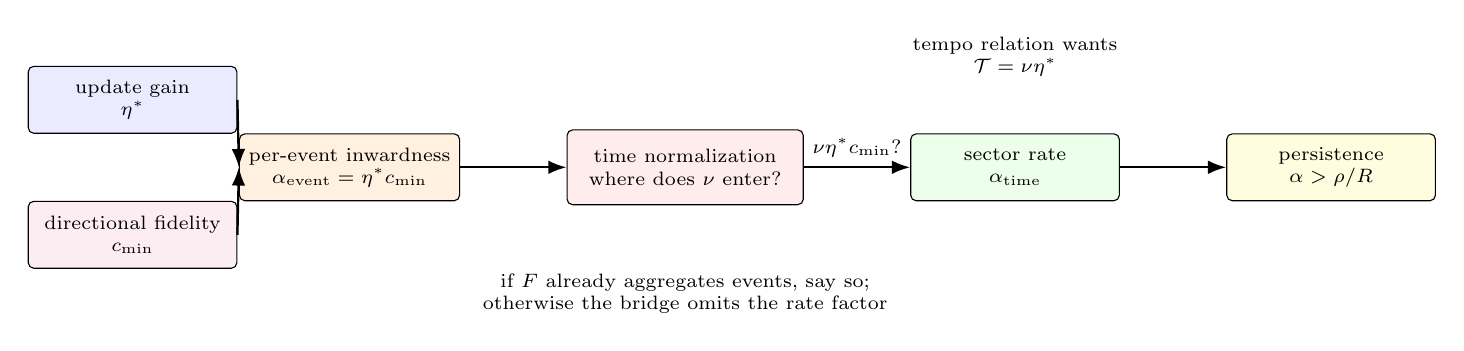
\begin{tikzpicture}[
  box/.style={draw, rounded corners=2pt, align=center, minimum width=2.65cm, minimum height=0.85cm, font=\scriptsize},
  warn/.style={draw, rounded corners=2pt, align=center, minimum width=3.0cm, minimum height=0.95cm, font=\scriptsize, fill=red!7},
  note/.style={align=center, font=\scriptsize},
  arr/.style={-Latex, thick},
  dasharr/.style={-Latex, thick, dashed}
]

\node[box, fill=blue!8] (gain) {update gain\\$\eta^\ast$};
\node[box, fill=purple!7, below=0.85cm of gain] (fid) {directional fidelity\\$c_{\min}$};
\node[box, fill=orange!12, right=1.35cm of $(gain)!0.5!(fid)$] (eventalpha)
  {per-event inwardness\\$\alpha_{\rm event}=\eta^\ast c_{\min}$};
\draw[arr] (gain.east) -- (eventalpha.west);
\draw[arr] (fid.east) -- (eventalpha.west);

\node[warn, right=1.35cm of eventalpha] (time) {time normalization\\where does $\nu$ enter?};
\node[box, fill=green!8, right=1.35cm of time] (alpha)
  {sector rate\\$\alpha_{\rm time}$};
\node[box, fill=yellow!12, right=1.35cm of alpha] (persist)
  {persistence\\$\alpha>\rho/R$};

\draw[arr] (eventalpha) -- (time);
\draw[arr] (time) -- node[above, font=\scriptsize] {$\nu\eta^\ast c_{\min}$?} (alpha);
\draw[arr] (alpha) -- (persist);

\node[note, below=0.75cm of time] {if $F$ already aggregates events, say so;\\otherwise the bridge omits the rate factor};
\node[note, above=0.6cm of alpha] {tempo relation wants\\$\mathcal T=\nu\eta^\ast$};

\end{tikzpicture}
\end{document}
